% SBI / FMPE workflow: simulate offline -> train flow -> amortized one-pass query.
% Compile:   pdflatex sbi_workflow.tex
% Rasterize: pdftoppm -png -r 300 sbi_workflow.pdf raw \
%            && magick raw-1.png -trim +repage sbi_workflow.png
\documentclass{article}
\usepackage[paperwidth=23cm, paperheight=8cm, margin=3mm]{geometry}
\usepackage{tikz}
\usepackage{amsmath}
\usepackage{amssymb}
\usepackage{bm}
\usetikzlibrary{positioning, arrows.meta, backgrounds, fit, calc}
\pagestyle{empty}

\definecolor{cSim}{HTML}{1F77B4}    % simulate (blue, uses solver)
\definecolor{cTrain}{HTML}{6A51A3}  % train flow (purple)
\definecolor{cInfer}{HTML}{D62728}  % inference (red)
\definecolor{cStage}{HTML}{90A4AE}

\begin{document}
\noindent
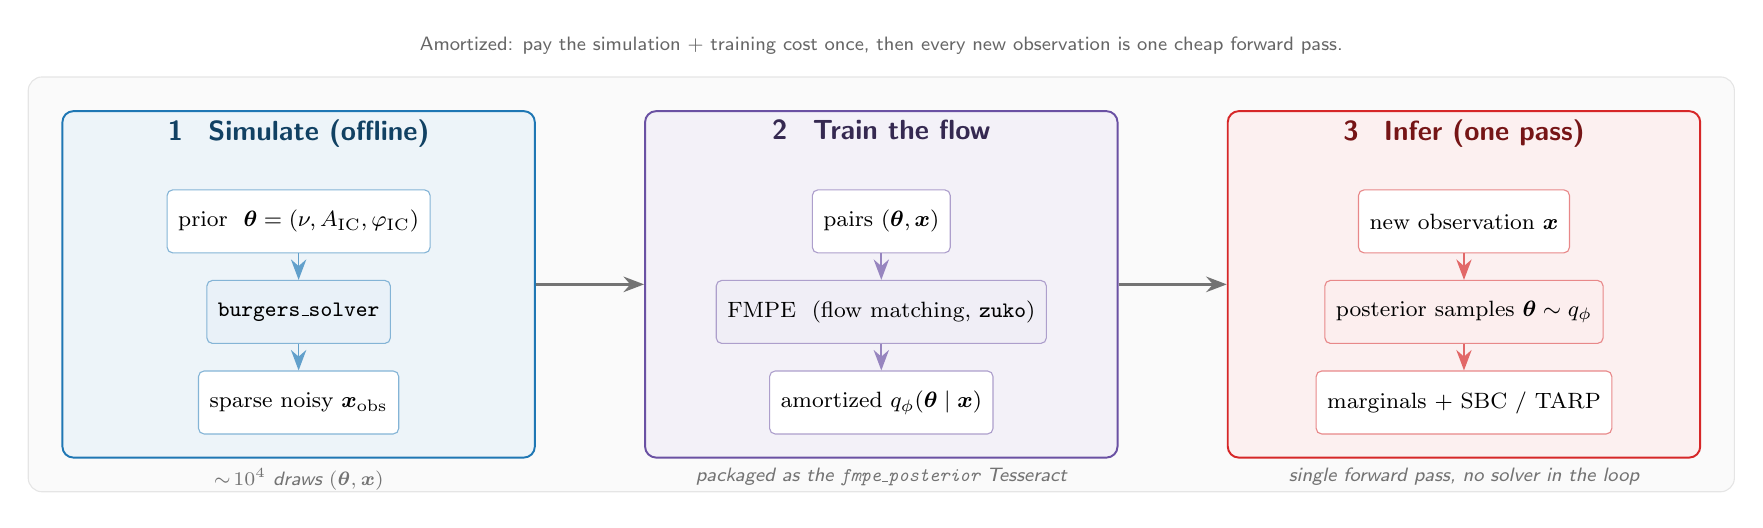
\begin{tikzpicture}[
  font=\sffamily,
  >={Stealth[length=2.6mm]},
  stage/.style={rounded corners=4pt, line width=0.7pt, align=center,
                minimum width=60mm, minimum height=44mm, inner sep=7pt},
  pill/.style={rounded corners=2pt, draw=black!35, fill=white,
               align=center, font=\footnotesize, inner sep=4pt,
               minimum height=8mm},
  big/.style={->, draw=black!55, line width=1.3pt},
  small/.style={->, draw=black!45, line width=0.6pt},
  head/.style={font=\sffamily\bfseries},
  note/.style={font=\sffamily\scriptsize\itshape, text=black!55},
]

% ====================== Stage 1: simulate (offline) ====================
\node[stage, fill=cSim!8, draw=cSim] (s1) at (0,0) {};
\node[head, text=cSim!55!black, anchor=north] at (s1.north) {1 \, Simulate (offline)};
\node[pill, draw=cSim!55] (prior) at (0,0.8)
  {prior \ $\bm{\theta}=(\nu, A_{\mathrm{IC}}, \varphi_{\mathrm{IC}})$};
\node[pill, draw=cSim!55, fill=cSim!10] (solv) at (0,-0.35)
  {\texttt{burgers\_solver}};
\node[pill, draw=cSim!55] (xobs) at (0,-1.5)
  {sparse noisy $\bm{x}_{\mathrm{obs}}$};
\draw[small, draw=cSim!70] (prior) -- (solv);
\draw[small, draw=cSim!70] (solv) -- (xobs);
\node[note, anchor=north] at (s1.south) {$\sim\!10^4$ draws $(\bm{\theta},\bm{x})$};

% ====================== Stage 2: train the flow ========================
\node[stage, fill=cTrain!8, draw=cTrain] (s2) at (7.4,0) {};
\node[head, text=cTrain!50!black, anchor=north] at (s2.north) {2 \, Train the flow};
\node[pill, draw=cTrain!55] (pairs) at (7.4,0.8)
  {pairs $(\bm{\theta},\bm{x})$};
\node[pill, draw=cTrain!55, fill=cTrain!10] (fmpe) at (7.4,-0.35)
  {FMPE \ (flow matching, \texttt{zuko})};
\node[pill, draw=cTrain!55] (qnet) at (7.4,-1.5)
  {amortized $q_\phi(\bm{\theta}\mid\bm{x})$};
\draw[small, draw=cTrain!70] (pairs) -- (fmpe);
\draw[small, draw=cTrain!70] (fmpe) -- (qnet);
\node[note, anchor=north] at (s2.south) {packaged as the \texttt{fmpe\_posterior} Tesseract};

% ====================== Stage 3: amortized inference ===================
\node[stage, fill=cInfer!7, draw=cInfer] (s3) at (14.8,0) {};
\node[head, text=cInfer!55!black, anchor=north] at (s3.north) {3 \, Infer (one pass)};
\node[pill, draw=cInfer!55] (newx) at (14.8,0.8)
  {new observation $\bm{x}$};
\node[pill, draw=cInfer!55, fill=cInfer!8] (post) at (14.8,-0.35)
  {posterior samples $\bm{\theta}\sim q_\phi$};
\node[pill, draw=cInfer!55] (diag) at (14.8,-1.5)
  {marginals $+$ SBC / TARP};
\draw[small, draw=cInfer!70] (newx) -- (post);
\draw[small, draw=cInfer!70] (post) -- (diag);
\node[note, anchor=north] at (s3.south) {single forward pass, no solver in the loop};

% ====================== between-stage arrows ===========================
\draw[big] (s1.east) -- (s2.west);
\draw[big] (s2.east) -- (s3.west);

% banner
\node[note, text=black!60, anchor=south] at (7.4,2.8)
  {\emph{Amortized: pay the simulation + training cost once, then every new
   observation is one cheap forward pass.}};

\begin{scope}[on background layer]
  \node[rounded corners=5pt, fill=black!2, draw=black!10,
        fit=(s1)(s2)(s3), inner sep=12pt] {};
\end{scope}

\end{tikzpicture}
\end{document}
